%%%%%%%%%%%%%%%%%%%% author.tex %%%%%%%%%%%%%%%%%%%%%%%%%%%%%%%%%%%
%
% template for chapters to the Handbook of Exoplanets
% modified by H. Deeg from the 'template.tex' provided by Springer for the svmult.cls class
% 20Mar 2016
%
%%%%%%%%%%%%%%%% Springer %%%%%%%%%%%%%%%%%%%%%%%%%%%%%%%%%%


% RECOMMENDED %%%%%%%%%%%%%%%%%%%%%%%%%%%%%%%%%%%%%%%%%%%%%%%%%%%
\documentclass[graybox,natbib,nosecnum]{svmult}
\bibpunct{(}{)}{;}{a}{}{,} % suppress commas between author-names and year

\pdfoutput=1   %forces use of pdflatex. Disable if you prefer to use .eps or .ps figures.
% choose options for [] as required from the list
% in the Reference Guide

\usepackage{mathptmx}       % selects Times Roman as basic font
\usepackage{helvet}         % selects Helvetica as sans-serif font
\usepackage{courier}        % selects Courier as typewriter font
\usepackage{type1cm}        % activate if the above 3 fonts are
                            % not available on your system

\usepackage{makeidx}         % allows index generation
\usepackage{graphicx}        % standard LaTeX graphics tool
                             % when including figure files
\usepackage{multicol}        % used for the two-column index
\usepackage[bottom]{footmisc}% places footnotes at page bottom
\usepackage[normalem]{ulem}	% for strike-through of text with \sout{}  
\usepackage{hyperref}  %for hyperlinks

\usepackage{soul}   % for high-lighting of text
% see the list of further useful packages
% in the Reference Guide

% expansions of  journal abbreviations from bibtex entries by ADS
% adapted to Springer Basic style (no periods in abbreviations)
\newcommand*\aap{A\&A}
\let\astap=\aap
\newcommand*\aapr{A\&A Rev}
\newcommand*\aaps{A\&AS}
\newcommand*\actaa{Acta Astron}
\newcommand*\aj{AJ}
\newcommand*\ao{Appl Opt}
\let\applopt\ao
\newcommand*\apj{ApJ}
\newcommand*\apjl{ApJ}
\let\apjlett\apjl
\newcommand*\apjs{ApJS}
\let\apjsupp\apjs
\newcommand*\aplett{Astrophys Lett}
\newcommand*\apspr{Astrophys Space Phys Res}
\newcommand*\apss{Ap\&SS}
\newcommand*\araa{ARA\&A}
\newcommand*\azh{AZh}
\newcommand*\baas{BAAS}
\newcommand*\bac{Bull astr Inst Czechosl}
\newcommand*\bain{Bull Astron Inst Netherlands}
\newcommand*\caa{Chinese Astron Astrophys}
\newcommand*\cjaa{Chinese J Astron Astrophys}
\newcommand*\fcp{Fund Cosmic Phys}
\newcommand*\gca{Geochim Cosmochim Acta}
\newcommand*\grl{Geophys Res Lett}
\newcommand*\iaucirc{IAU Circ}
\newcommand*\icarus{Icarus}
\newcommand*\jcap{J Cosmology Astropart Phys}
\newcommand*\jcp{J Chem Phys}
\newcommand*\jgr{J Geophys Res}
\newcommand*\jqsrt{J Quant Spectr Rad Transf}
\newcommand*\jrasc{JRASC}
\newcommand*\memras{MmRAS}
\newcommand*\memsai{Mem Soc Astron Italiana}
\newcommand*\mnras{MNRAS}
\newcommand*\na{New A}
\newcommand*\nar{New A Rev}
\newcommand*\nat{Nature}
\newcommand*\nphysa{Nucl Phys A}
\newcommand*\pasa{PASA}
\newcommand*\pasj{PASJ}
\newcommand*\pasp{PASP}
\newcommand*\physrep{Phys Rep}
\newcommand*\physscr{Phys Scr}
\newcommand*\planss{Planet Space Sci}
\newcommand*\pra{Phys Rev A}
\newcommand*\prb{Phys Rev B}
\newcommand*\prc{Phys Rev C}
\newcommand*\prd{Phys Rev D}
\newcommand*\pre{Phys Rev E}
\newcommand*\prl{Phys Rev Lett}
\newcommand*\procspie{Proc SPIE}
\newcommand*\qjras{QJRAS}
\newcommand*\rmxaa{Rev Mexicana Astron Astrofis}
\newcommand*\skytel{S\&T}
\newcommand*\solphys{Sol Phys}
\newcommand*\sovast{Soviet Ast}
\newcommand*\ssr{Space Sci Rev}
\newcommand*\zap{ZAp}


\newcommand{\hbindex}[1]{\hl{#1}\index{#1}}  %highlights index entries

\newcommand{\project}[1]{\textsl{#1}}
\newcommand{\JWST}{\project{JWST}}
\newcommand{\HST}{\project{HST}}
\newcommand{\TESS}{\project{TESS}}
\newcommand{\Spitzer}{\project{Spitzer}}
\newcommand{\Kepler}{\project{Kepler}}


\makeindex             % used for the subject index
                       % please use the style svind.ist with
                       % your makeindex program

%%%%%%%%%%%%%%%%%%%%%%%%%%%%%%%%%%%%%%%%%%%%%%%%%%%%%%%%%%%%%%%%%%%%%%%%%%%%%%%%%%%%%%%%%

\begin{document}

\title*{Exoplanet Atmosphere Measurements from Transmission Spectroscopy and other Planet-Star Combined Light Observations}
\titlerunning{Atmosphere Measurements from Combined Light Observations} 
% Use \titlerunning{Short Title} for an abbreviated version of
% your contribution title if the original one is too long
\author{Laura Kreidberg}
% Use \authorrunning{Short Title} for an abbreviated version of
% your contribution title if the original one is too long
\institute{Laura Kreidberg \at Harvard Society of Fellows, 78 Mount Auburn Street, Cambridge, MA, 02138, \email{laura.kreidberg@cfa.harvard.edu}}
%
% Use the package "url.sty" to avoid
% problems with special characters
% used in your e-mail or web address
%
\maketitle


\abstract{Abstract.}

\section{The Promise of Exoplanet Atmospheres}
Exoplanet atmospheres are a treasure trove of information. By measuring the chemical composition and thermal structure of an atmosphere, it is possible to constrain the planet's formation and evolutionary history, current climate, and even habitability.  Making good on this opportunity is challenging on a technical level, however. In most cases, it is not possible to spatially resolve the planet from its host star, and the star outshines the planet by a factor of at least a thousand to one. 

The subject of this chapter is atmosphere characterization through analysis of the combined light from the planet and the star. This approach is best suited to transiting planets, which periodically pass in front of and behind their host stars. During a transit, a small fraction of the stellar light filters through the planet's atmosphere on its path to us. When the planet is eclipsed, its thermal emission and reflection are blocked.  With meticulous observations, these effects can be measured relative to the constant baseline flux from the star. The resulting inferences of planetary atmospheric properties can be remarkably detailed, given that they were based solely on point sources of light hundreds of parsecs distant.

In this chapter, we review combined light observing techniques, discuss current observational facilities and best practices, and highlight major science results.

\section{Observing Techniques} 

\subsection{Transit Spectroscopy}
The most widely used combined-light technique is transmission spectroscopy. For this method, the planet is observed in transit as it passes in front of its host star, as illustrated in Figure\,\ref{fig:geom}.  The measurement of total (star plus planet) brightness over time is known as the transit light curve.  During the transit, the planet blocks a small fraction of the stellar flux equal to the sky-projected area of the planet relative to the area of the star. We refer to this fractional drop in flux as the \hbindex{transit depth}, $\delta$. 

\begin{figure}
\begin{centering}
\includegraphics[scale=.4]{Figures/transit_geom.pdf}
\caption{Illustration of transit and eclipse geometry. Over the course of the planet's orbit, it periodically passes in front of the star (a transit event) and behind (a secondary eclipse). A few key distances are labeled: the planet and stellar radii, $R_p$ and $R_s$, the atmospheric scale height $H$, and the separation of centers in the plane of the sky, $d$. Figure adapted from FIXME.}
\label{fig:geom}       
\end{centering}
\end{figure}

The key idea behind transmission spectroscopy is that the planet's transit depth is \emph{wavelength-dependent}.  At wavelengths where the atmosphere is relatively more opaque due to absorption by atoms or molecules, the planet blocks slightly more stellar flux.  To measure these variations, the light curve is binned in wavelength into spectrophotometric channels, and the light curve from each channel is fit separately with a transit model.  The measured transit depths as a function of wavelength constitute the \hbindex{transmission spectrum}, so named because it arises from the transmission of stellar flux through the planet's atmosphere.
 
\begin{figure}
\begin{centering}
\includegraphics[scale=.8]{Figures/w12_lc.pdf}
\caption{Transit light curve measured with the Hubble Space Telescope for the hot Jupiter WASP-12b \citep{kreidberg15b}. The systematics-corrected data (points) are shown in the top panel compared to the best fit transit model (line). The data are color coded by the observation date. Gaps in coverage are due to Earth occultation. The middle panel shows the residuals from the best fit, and the bottom panel show a histogram of the residuals compared to the expected photon noise.}
\label{fig:lc}       
\end{centering}
\end{figure}

Theoretical models for the transmission spectrum require radiative transfer calculation for light on the slant path through the atmosphere \citep{seager00}, a computationally intensive task. However, we can make a rough prediction of the size of features in the transmission spectrum based on the atmospheric \hbindex{scale height} $H$. The scale height is the change in altitude over which the pressure drops by a factor of $e$. Assuming hydrostatic equilibrium, 

\begin{equation}
H = \frac{K_bT_{eq}}{\mu g}
\end{equation}
where $K_b$ is the Boltzmann constant, $T_{eq}$ is the planet's \hbindex{equilibrium temperature}, $\mu$ is the mean molecular mass, and $g$ is the surface gravity.

The amplitude of spectral features in transmission is then:
\begin{eqnarray}
\delta_\lambda &=& \frac{(R_p + nH)^2}{R_s^2} - \frac{R_p^2}{R_s^2}\\
 & \approx & 2R_pH/R_s^2
\end{eqnarray} 
where $n$ is the number of scale heights crossed at wavelengths with high opacity (typically around two for cloud-free atmospheres; \cite{stevenson16}. The ideal candidates for transmission spectroscopy is a planet with high equilibrium temperature, a small host star, low surface gravity, and a low mean molecular mass atmosphere. Even for these ideal cases, however, the amplitude of spectral features is just $\delta_\lambda \sim0.1\%$ \citep[e.g. WASP 121-b;][]{evans16}. For Earth-like planets, the expected amplitude is two to three orders of magnitude smaller, depending on host star size. 

\begin{figure}
\begin{centering}
\includegraphics[scale=.8]{Figures/w43.pdf}
\caption{Thermal emission and transission spectra for the hot Jupiter WASP-43b \citep{kreidberg14b}. Water absorption FIXME: permissions.} 
\label{fig:spectra}       
\end{centering}
\end{figure}

Theoretical models for the transmission spectrum require radiative transfer calculation for light on the slant path through the atmosphere \citep{seager00}, a computationally intensive task. However, we can make a rough prediction of the size of features in the transmission spectrum based on the atmospheric \hbindex{scale height} $H$. The scale height is the change in altitude over which the pressure drops by a factor of $e$. Assuming hydrostatic equilibrium, 


\subsection{Occultation Spectroscopy}
A close cousin of the transit spectroscopy method is \hbindex{occultation spectroscopy}, which measures thermal emission and reflection from the planet. Rather than observing the planet during transit, it is observed at secondary eclipse, when it passes behind the host star. The eclipse provides a baseline measurement of the stellar flux alone. When the planet rotates back into view, any increase in brightness can be attributed to the planet's thermal emission and reflected light.

\runinhead{Thermal Emission}
For the short-period planets that have been studied so far, the dominant source of thermal emission is re-radiation of incident stellar flux (rather than latent heat of formation, as seen for directly imaged planets). Thus the typical size of the emission signal can be predicted from the planet's equilibrium temperature:

\begin{equation}
\label{eqn:fpfs}
\frac{F_p}{F_s} = \frac{B(\lambda, T_{eq})}{B(\lambda, T_s)}\left(\frac{R_p}{R_s}\right)^2
\end{equation}
where $F_p/F_s$ is the planet-to-star flux ratio, $B(\lambda, T)$ is the blackbody spectral radiance at temperature $T$, and $R_p/R_s$ is the planet-to-star radius ratio. Since the planet is cooler than the star, the flux ratio is larger at longer wavelengths. For example, the planet-to-star flux for the hot Jupiter HD 209458b is just 50 parts per million at 1 $\mu$m, but increases to over 1000 ppm at 4.5 $\mu$m \citep{line16}.

Equation \ref{eqn:fpfs} is a good first order approximation of the planet signal, but as with transmission spectroscopy, more complex features arise in the spectrum due to the atmosphere's changing opacity with wavelength. The emitted light comes from the photosphere of the planet, where the optical depth is of order unity. At more opaque wavelengths, the photosphere is at higher altitude, where the temperature may be cooler than $T_\mathrm{eq}$. The emission spectrum is therefore sensitive to both atmosphere's opacity \emph{and} its thermal structure. 

%A useful way to describe the temperature of the photosphere is the \hbindex{brightness temperature}: the temperature a blackbody needed to replicate the observed spectral intensity at a given wavelength.

\runinhead{Reflected Light}
At short wavelengths, reflected light from the planet may also be detectable. It is convenient to quantify the amount of reflected light in terms of a ``perfect" mirror: a flat, reflecting disk with the same cross-sectional area as the planet. The ratio of reflected light from the fully illuminated planet, relative to reflection by a perfect mirror, is the geometric albedo $A_g$. The total reflected light signal is

\begin{equation}
F_{reflect} = A_g(R_p/a)^2 \Phi(\alpha)
\end{equation}
where $a$ is the orbital separation and $\Phi(\alpha)$ is the phase function (the reflected light intensity at phase angle $\alpha$). The phase function depends on the scattering properties of the atmosphere, but analytic predictions are available for certain simplified models \citep[e.g.][]{madhu12}.  Reflected light is easiest to detect in the optical, where it dominates the thermal emission signal; however, the amplitude tends to be small \citep[typically less than 100 ppm;][]{angerhausen15}.

\runinhead{Phase Curves}
In addition to characterizing thermal emission and reflected light from secondary eclipses, it is also possible to observe a full-orbit \hbindex{phase curve}. These observations consists of continuous time series photometry or spectroscopy of a planet over its entire orbital period, using the secondary eclipse as a baseline measurement of the stellar flux alone.  The best targets for phase curves are short-period planets that are tidally locked to their host stars. For these planets, the rotation period is known (equal to their orbital period), so over the course of one complete orbit all longitudes are visible in turn.  Phase curve observations are powerful because they probe atmospheric physics and chemistry over a wider geographic region than transits or eclipses. %However, they are challenging from a technical standpoint because they require long stares at a single object. %In principle it is possible to apply this technique to longer period planets that are not tidally locked; however, in addition to the feasibility challenge the interpretation is also problematic. 

\runinhead{Eclipse Mapping}
All of the occultation spectroscopy techniques described above rely on a hemisphere average of the planet's reflected or emitted light. To glean additional spatial information, one can use the \hbindex{eclipse mapping} method, which requires precise observations of the secondary eclipse light curve during ingress and egress.  During these intervals, the hemisphere of the planet is partially eclipsed by the star, allowing the observer to pinpoint the brightness of a smaller region and thus map the brightness distribution in detail \citep{rauscher07}.  This is the only combined light technique that is sensitive to the planet's brightness as a function of \emph{latitude} (because higher latitudes are first to enter and exit eclipse).
% This approach is based on the fact that planets are not uniformly bright. In the case of a hot gas giant, the hottest part of the atmosphere may be offset from the substellar point due to atmospheric circulation. For a terrestrial planet, continents and oceans with varying reflectivity may be present. 


%\runinhead{Hubble Space Telescope}
%The 2.7 m \emph{Hubble Space Telescope} (\HST) has two instruments widely used for atmosphere studies: the \hbindex{Wide Field Camera 3} (WFC3) and the \hbindex{Space Telescope Imaging Spectrograph} (STIS).  WFC3 is \HST's newest detector (installed in 2009) and succeeds NICMOS (the Near Infrared Camera and Multi-Object Spectrometer). It provides near-infrared, low-resolution spectroscopy from $0.8 - 1.7$ $\mu$m, where water molecules have strong absorption features.  STIS has complementary capabilities: it is a UV/optical instrument sensitive to the wavelength range $0.1 - 1 \, \mu$m. This range covers absorption lines from atomic alkali metals, as well as the Lyman-$\alpha$ transition of atomic hydrogen. 


%\runinhead{Spitzer Space Telescope}
%In addition to \HST, the other space-based observing facility is \Spitzer, an 85 cm telescope launched in 2003. \Spitzer\ provided infrared spectroscopy from 3 - 160 $\mu$m until 2009, when it ran out of coolant. Now operating in its Warm Mission, \Spitzer\ is currently capable of broadband photometry at 3.6 and 4.5 $\mu$m with the \hbindex{Infrared Array Camera} (IRAC).  \Spitzer's unique strength is its long wavelength coverage, where planet-to-star flux ratios are higher. It is therefore often used for thermal emission measurements. \Spitzer\ also provides continuous observing capability thanks to its heliocentric orbit, and has led the way in long-duration observations of thermal phase curves \citep[e.g.][]{knutson07}. 

%\subsection{Ground-based}
%The two main ground-based observing techniques -- low-resolution spectroscopy with wide slits and high resolution observations -- both require specialized instruments. For the wide slit approach, there are only a few observatories that have multi-object spectrographs with a custom slit mask option. Several that have been used for exoplanet observations are VLT/FORS2, Magellan/IMACS, Keck/MOSFIRE, MMT/MMIRS, Gemini/GMOS, and Magellan/LDSS3-C \citep{bean10, jordan13, crossfield13, bean13, stevenson14c, stevenson16b}.

%The high resolution technique also requires specific capabilities: resolution $R\sim100000$ to detect individual spectral lines, as well as high S/N over wavelength regions with many lines. Most detections using this technique have come from VLT/CRIRES \citep[e.g.][]{snellen10}.  Keck/NIRSPEC and HARPS have also been used \citep{lockwood14, martins15}.  
%\subsection{Reliability}


%\section{Best Practices for Achieving Precise and Accurate Measurements}
%The basic format for observing transiting planets is time series spectroscopy or photometry, with the goal of detecting small deviations in brightness over time due to the planet's orbital motion.  In this section we summarize a few good practices and discuss sources of error (both astrophysical and instrumental).

%\subsection{Light Curve Fitting} 
%The reduced data consist of a time series of brightness measurements (either a ``white" light curve summed up over the entire bandpass, or spectroscopic light curves created by binning the spectrum into channels).  The most general model for the data is:

%\begin{equation}
%F(t) = S(t) \times T(t) \times E(t) \times \phi(t)
%\end{equation}
%where $S(t)$ is the systematics model (for signals that are not astrophysical; e.g., a linear trend with time), $T(t)$ is the transit model, $E(t)$ is the eclipse, and $\phi(t)$ is the phase variation from reflected and emitted light. In cases where only a transit or eclipse is observed, the phase variation can usually be neglected.

%FIXME: rewrite this paragraph. Transit and eclipse models both depend on the planet's orbital position as a function of time. This is the classic two-body problem, solved in any dynamics textbook \citep[e.g.][]{murray99}. In addition to the orbital solution, the transit model also requires the planet-to-star radius ratio $R_p/R_s$ and the stellar brightness profile. Due to limb darkening, the stellar disk is brighter at the center than at the edge, so the fraction of flux blocked by the planet depends on its exact position.  \cite{mandel02} and \cite{gimenez06} calculated analytic solutions for the transit light curve for a range of stellar brightness profiles,  which are implemented in a number of publicly available software packages including \texttt{JKTEBOP}, \texttt{TAP}, \texttt{ExoFast}, \texttt{PyTransit}, and \texttt{batman} \citep{southworth04, gazak12, eastman13, parviainen15, kreidberg15a}.  FIXME say more about limb darkening.

%The physical parameters for the orbit are the period $P$, time of inferior conjunction $t_0$, orbital separation $a$, inclination $i$, eccentricity $e$.  The orbital solution can be obtained via Kepler's law \citep{murray99}.
%The eclipse model is a more straightforward calculation: 
%\begin{equation}
%E(t) = 1 + F_p/F_s (1 - \alpha(t)) 
%\end{equation}
%where $F_p/F_s$ is the planet-to-star flux ratio and $\alpha(t)$ is the fraction of the planet disk eclipsed by the star (easily calculated from the overlapping area of two circles). This model assumes the brightness of the planet is constant, and neglects planetary limb darkening or other variation in temperature/reflectivity. In practice, these variations are only detectable for the highest precision light curves \citep{FIXME}. 

%The planet's phase variation is typically fit using a sinusoid with period equal to the planet's orbital period, with the option of adding higher harmonics \citep[e.g.][]{knutson12, stevenson16}. Alternatively, one can fit an ``orange slice" model that assumes constant planet brightness over slices in longitude \citep{knutson07, cowan08}. 
%A third option is to create a physically motivated temperature map and calculate the \citep{zhang16}. 

%\subsection{Estimating Parameter Uncertainties}
%As for all measurements, correctly estimating the uncertainty on the planet spectrum is as important as the detection itself.  The best approach for determining the uncertainties depends primarily on whether the noise is correlated in time.  

%In the case of uncorrelated noise (referred to as ``white" or ``Gaussian" noise), the uncertainties can be estimated with the Markov chain Monte Carlo (MCMC) technique, a Bayesian method that calculates the posterior probability distribution for the model parameters (see \citealt{sivia96} for a general overview of Bayesian methods and \citealt{ford05} for a specific application of MCMC to exoplanets). These fits can be computationally challenging, especially if there are many parameters, correlated uncertainties, or multi-modal solutions. Sophisticated MCMC methods have been developed to address these issues, including differential evolution MCMC \citep{braak06}, or affine-invariant sampling \citep{goodman10}, implemented in the Python package \texttt{emcee} \citep{foremanmackey13}.

%Estimating uncertainties is more difficult in the presence of ``red", time-correlated noise, which is often present in ground-based light curves \citep{}. Red noise is easily identified by eye in the residuals of the light curve fit as time-dependent trends. To quantitatively test for it, one can bin the data points in time. If the noise is white, the residuals are expected to decrease proportionally to the square root of the number of data points per bin. If the binned residuals are larger than expected, red noise is present and needs to be accounted for in the model fit.  A number of strategies have been developed to model red noise, including ``residual permutation bootstrap" (also known as ``prayer bead")  \citep{southworth08}, wavelet-based methods \citep{carter09}, and Gaussian processes \citep{rasmussen05}. Depending on the amplitude of the red noise, it can increase parameter uncertainties by factors of several, so it must be treated carefully.

\section{Practical Considerations}
Detecting the tiny signals from exoplanet atmospheres is a formidable challenge. Even for the most favorable systems, the amplitude of spectral features is of order a tenth of a percent. Pushing to this level of precision requires many photons (and thus large telescopes), a stable observing environment, and detailed knowledge of the planet's host star.  In this section, we summarize the state-of-the-art in observing facilities, briefly review ground-based observing techniques, and discuss possible sources of error.

\subsection{Observing Facilities}
The Hubble and Spitzer Space Telescopes are the preeminent facilities for exoplanet atmosphere studies.  Space-based observations have several advantages: they are free from atmospheric turbulence that adds systematic noise to light curves, they can access wavelengths where the Earth's atmosphere is strongly absorbing (e.g., ultra-violet and water absorption bands), and detectors can be cooled to low temperatures, enabling longer wavelength observations than are possible from the ground.  

As of 2017, the workhorse instruments for atmosphere characterization are the Space Telescope Imaging Spectrograph (STIS) and the Wide Field Camera 3 (WFC3) on board Hubble, and Spitzer's Infrared Array Camera (IRAC).  These instruments provide spectroscopy from the UV to the near-infrared (ending at 1.7 $\mu$m), and broadband photometry at 3.6 and 4.5 $\mu$m. The suite of instruments built for the James Webb Space Telescope (JWST; scheduled for launch in 2018), will provide significantly expanded spectroscopic coverage, from $0.6$ to $12\,\mu$m.  Figure FIXME illustrates the observing capabilities of these current and planned instruments. 

\subsection{Ground-Based Observations}
Exoplanet atmosphere characterization is possible from the ground, but it is challenging because
the transparency of Earth's atmosphere changes with time.  As a target moves through the sky, line-of-sight properties such as the airmass, precipitable water vapor, and cloud coverage will vary, introducing systematic trends in the light curve that may be orders of magnitude larger than the signal from the planet. 

To correct for these effects, one approach is to use comparison stars to correct for systematic trends in the target light curve. In addition to the target, several nearby stars are observed in the same field of view. The path of their flux traverses similar parts of the Earth's atmosphere, so their light curves exhibit nearly identical systematic trends as the target. The target light curve can then be divided by the sum of the comparison star light curves to remove systematics.  For spectroscopic observations, the target and comparison stars must be observed with a custom-made mask with wide slits ($>10''$) to avoid time-dependent slit losses due to variable seeing, a technique developed by \cite{bean10}.

Another creative ground-based technique uses high resolution spectroscopy to detect the planet's atmosphere.  The idea is that the planet spectrum is Doppler shifted due to its orbital motion, and thus separated in wavelength from both the stellar spectrum and telluric lines from the Earth's atmosphere. The planet spectrum can be cross-correlated with a template to reveal the atmospheric composition and orbital velocity \citep[e.g.][]{snellen10}.  This technique is discussed in detail in Chapter FIXME. 

\subsection{Noise Sources}
\runinhead{Random}
\hbindex{Photon noise} is the fundamental limit on the precision of a light curve. A star emits $N \pm \sqrt{N}$ photons per unit time. The $\sqrt{N}$ noise arises because each atom in the star emits a photon with some small probability, so the total number emitted per time interval follows a Poisson distribution. The relative error ($\sqrt{N}/N$) decreases as $N$ increases, so bright stars yield more precise light curves.  The best target systems for atmosphere characterization typically have H mag $< 10$ for infrared observations.  The precision of a light curve is often quantified by how close it is to the photon-limited noise floor. Space-based observations often reach the photon limit \citep{sing11, kreidberg14a, ingalls16}, whereas ground-based observations are typically a factor of a few above it \citep[e.g.][]{bean13}. 

\runinhead{Instrument Systematics}
Instrument-based systematics are a major source of error in precise time series photometry. They can be orders of magnitude larger than the planet signal. Two common systematic effects are: 

\begin{itemize}
\item{\emph{Charge trapping}. Near-infrared detectors (e.g. \HST/WFC3) have impurities that can trap photoelectrons \citep{smith08}. As the traps fill up exponentially over time, the observed count rate increases by a factor of approximately $1 - R e^{-t/\tau}$, where $R$ and $\tau$ depend on the detector and illumination level.  This same mechanism is responsible for image persistence, the afterglow the appears as charge traps are released. The effect can be corrected with analytic models to photon-limited precision \citep{deming13, line16}. 
}
\item{\emph{Intrapixel effect.} Detector pixels do not have perfectly uniform spatial sensitivity, so the measured flux is correlated with the $X, Y$ position of the centroid of the image. This effect is the dominant systematic error for infrared measurements (e.g. \Spitzer/IRAC). Many techniques have been developed to model intrapixel variation, including \texttt{BLISS} mapping \citep{stevenson12}, pixel-level decorrelation \citep{deming15}, and ICA \citep{morello15}.}
\end{itemize}

\runinhead{Astrophysical Systematics}
Systematic errors also arise from incorrect or incomplete models for the stellar or planet flux. These include: 

\begin{itemize}
\item{\emph{Background stars.} Roughly half of stars have one or more bound companions \citep{raghavan10}. If the companion flux is blended with that of the host star, it dilutes the planet signal. Transit and eclipse depths must be multiplied by a correction factor $1 + \beta(\lambda)$ where $\beta$ is the ratio of the background star to host star flux. High contrast imaging is needed to detect close companions, and should be obtained for systems that are targets for atmosphere characterization.}
\item{\emph{Star spots.} To first order, the temperature difference between the stellar photosphere and the spotted region introduces a slope in the planet spectrum. If the spots are cool enough for molecules to form (e.g. water), they can even produce spurious spectral features, as there is no way to distinguish between absorption due to the spot and absorption by the planet atmosphere. The effect from spots can be corrected by multiplying the planet spectrum by a factor $(1-s\times[1-F_{\lambda,\mathrm{spot}}/F_{\lambda,\mathrm{phot}}])^{-1}$, where $s$ is the spot covering fraction and $F_\lambda$ is spectral radiance for the spot or the photosphere \citep{mccullough14}. The spot properties can be estimated based on the amplitude of long-term photometric variability in the stellar lightcurve or from spot crossing during transit \citep[e.g.][]{pont08}.} 
\item{\emph{Stellar activity.} Variations in star spot coverage are also a source of bias in transit depth measurements. To correct transit depths taken at different epochs, one can obtain photometric monitoring of the host star to estimate changes in $s$ and correct the depths with the above scale factor.} 
\item{\emph{Nightside emission from the planet.} For the hottest planets, thermal emission from the nightside may contribute significant flux during the transit. The nightside temperature depends on the planet's heat redistribution and cloud coverage, so can only be measured directly from phase curve observations. To correct for nightside flux, the transit depths should be multiplied be a factor FIXME \citep{kipping10}.} 
\end{itemize}

\runinhead{Notes on Reliability}
As we discussed in this section, there are many potential pitfalls in precise atmosphere characterization, and several early results were later disputed \citep[e.g.][]{tinetti07, swain08, gibson11}. However, in recent years, sophisticated data analysis and observing techniques have produced Hubble and Spitzer results that are photon noise-limited, repeatable, and reproducible by multiple teams \citep[e.g.][]{deming13, kreidberg14a, ingalls16}. The best achieved precision to date is 15 ppm on the emission spectrum of HD 209458b at a resolution $R\sim 30$ \citep{line16}, based on five secondary eclipse observations.

FIXME: say something about ground-based here.
%Ground-based observations have not been as thoroughly vetted as space-based data.  The comparison star technique can yield light curves that are within a factor of a few times the photon noise limit, but it is a challenge to estimate uncertainties correctly in the presence of residual correlated noise \citep[e.g.][]{jordan13, beatty16}.  

\section{Major Results from Atmosphere Studies}
In this section we discuss observational highlights, with a focus on space-based transmission and emission spectroscopy.  For recent comprehensive reviews, see \cite{crossfield15} and \cite{deming17}. 

\subsection{Atmospheric Composition}
\runinhead{Expectations}
We know from the Solar System that atmospheric composition can vary widely from planet to planet. Even so, we can still make educated guesses about possible compositions based on the building blocks of planet formation,  which come from disks of gas and dust surrounding young stars.  The protoplanetary disk has similar composition to the host star: predominantly hydrogen and helium, with smaller amounts of metals (the most abundant being oxygen, carbon, and nitrogen; \citealt{anders89}).  Planetary atmospheres can be made up directly from this material (so-called primary atmospheres, swept up during the accretion phase);  alternatively, secondary atmospheres may form on terrestrial planets by volcanic outgassing or delivery of volatiles by comets.  

At typical temperatures and pressures in planetary atmospheres, the dominant constituent elements (H, C, N, and O) are expected to combine into H$_2$, H$_2$O, CO, CO$_2$, CH$_4$, NH$_3$, O$_2$, and N$_2$.  In addition to these species, there are few trace atoms and molecules that may be detectable in a planet's spectrum thanks to their large absorption cross sections: namely, the alkali metals (sodium and potassium) and titanium and vanadium oxides (which may present at high temperatures; FIXME). In Figure FIXME, we show the predicted opacity of dominant absorbing species for an Earth-analog and a hot Jupiter. At any given wavelength, the absorber with the largest opacity will dominate the planet's spectrum.

%We note that in the nomenclature of planetary science, H$_2$ and He are referred to as \hbindex{gases}, and the other molecules are \hbindex{ices} \citep{depater15}.  
%The most abundant molecules are not necessarily the easiest to detect in a planet's spectrum, however. Observability depends on both abundance \emph{and} absorption cross-section. Hydrogen and helium, though they are the dominant component by mass for giant planet atmospheres, are relatively weak absorbers. By contrast, water and other ices have large absorption cross sections thanks to millions of rotational and vibrational line transitions between the optical and the far-infrared \citep{tennyson12}.  Ices are thus expected to dominate planets' spectra.  In addition, there are a few trace species with very large cross sections (alkali metals, titanium and vanadium oxides) that may be seen \citep{seager00, fortney08}.

\runinhead{Detections}
Many of the predictions listed above have been borne out.  The first detection of an absorbing species was the sodium resonance doublet at 589 nm in the hot Jupiter HD 209458b \citep{charbonneau02}. Since then, both sodium and potassium have been detected in a number of other hot Jupiters \citep[e.g.][]{sing11b, jensen11, nikolov14, fischer16}.

Hydrogen has also been detected, both in molecular and atomic form. \cite{lecavelier08} observed the signature of Rayleigh scattering from hydrogen in HD 209458b's optical transmission spectrum.  Lyman-$\alpha$ observations with HST/STIS revealed  large exospheres of escaping atomic hydrogen around hot planets \citep[e.g.][]{vidal-madjar03, ehrenreich15}.  These exospheres also contain ionized metals \citep[e.g., OI, CII][]{vidal-madjar04}. For more on atmospheric escape, see Chapter FIXME.

The most commonly observed molecular species is water, which has been seen in over a dozen planets \citep[e.g.][]{deming13, huitson13, mccullough14, fraine14, kreidberg14b, kreidberg15b, line16, evans16}. Most of these results come from \HST/WFC3 spectra in the near-IR (1.1 - 1.7 $\mu$m), where water is the dominant absorber. Water has also been detected from the ground \citep{birkby13, stevenson16b}.  Figure FIXME shows an example of water features in the transmission and emission spectra of WASP-43b \citep{kreidberg14b}. 

Carbon-bearing molecules have proven harder to detect, mainly due to the limitations of current observing facilities. CO has been detected a few times with high-resolution ground-based data \citep{dekok13,brogi14}.  There is also evidence for CO and CO$_2$ absorption in \Spitzer\ photometry \citep[e.g.][]{desert09}. However, the \Spitzer\ bandpasses are about $1\,\mu$m wide and cover spectral features from multiple different absorbing species (CO, CO$_2$, H$_2$O), making it a challenge to definitively identify which absorber is present. 

There have been tentative detections of several other molecules, including TiO, FeH, and HCN/NH$_3$ \citep[e.g.,][]{tsiaras16, evans16, macdonald17}. Future observations with broader spectral coverage and higher precision are needed to verify the presence of these absorbers.

We note that nearly all of the results listed here are for hot Jupiters, but there have been a few detections for smaller, cooler planets. Water features were inferred in the transmission spectra of two exo-Neptunes with equilibium temperatures below FIXME K \citep{fraine14, wakeford17}. The thermal emission spectrum of the warm Neptune GJ 436b shows a strong absorption feature in the Spitzer 4.5 $\mu$m filter, which could be due to CO/CO$_2$ \citep{morley17}. 

\runinhead{Absolute Abundances}
Once an atom or molecule has been detected, a next step is to measure its abundance. Abundance measurements are useful because they are diagnostic of planetary formation conditions, such as the surface density of solids and the relative accretion rates of gas and ice \citep[e.g.][]{fortney13, mordasini16}. Abundances are typically quantified in terms of their enrichment over the solar value (i.e., the expected abundance for a solar composition gas at the temperature of the planet's atmosphere).

The more precise the abundance measurement, the better it can constrain planet formation. However, precise determinations are challenging, even if molecular absorption is detected at high confidence.  Based on transmission spectra alone, there are order of magnitude degeneracies between chemical mixing ratios and atmospheric pressure \citep{benneke12, griffith13, kreidberg15b}.  

To break this degeneracy, one approach is to observe the planet's thermal emission.  Emission spectra are more sensitive to absolute abundance because the shape and amplitude of spectral features depend on the temperature-pressure profile. For example, \cite{stevenson17} measured the water abundance for the hot Jupiter WASP-43b to better than a factor of five  ($0.3 - 1.7\times$ solar at $1\,\sigma$ confidence). Another technique to improve precision requires observe multiple absorption bands for the same molecule in transmission \citep{benneke12}.  \cite{wakeford17} detected two water features in the transmission spectrum of the warm Neptune HAT-P-26b and retrieved a water abundance of $0.8 - 26\times$ solar at 1\,$\sigma$ \citep{wakeford17}.

These abundance measurements show intriguing tension with the Solar System trend, where atmospheric metallicity increases with decreasing planet mass. This trend is a natural outcome of planet population synthesis models, which show that lower mass planets are relatively more polluted by infalling planetesimals \citep{fortney13, mordasini16}. As shown in Figure FIXME, the metallicity of WASP-43b agrees with the Solar System pattern, but HAT-P-26b is less enriched than Uranus and Neptune. These results hint at the diversity of atmospheric compositions that exist beyond the Solar System, and provide a proof of concept that precise abundance measurements are possible for exoplanets. 
 
\begin{figure}
\begin{centering}
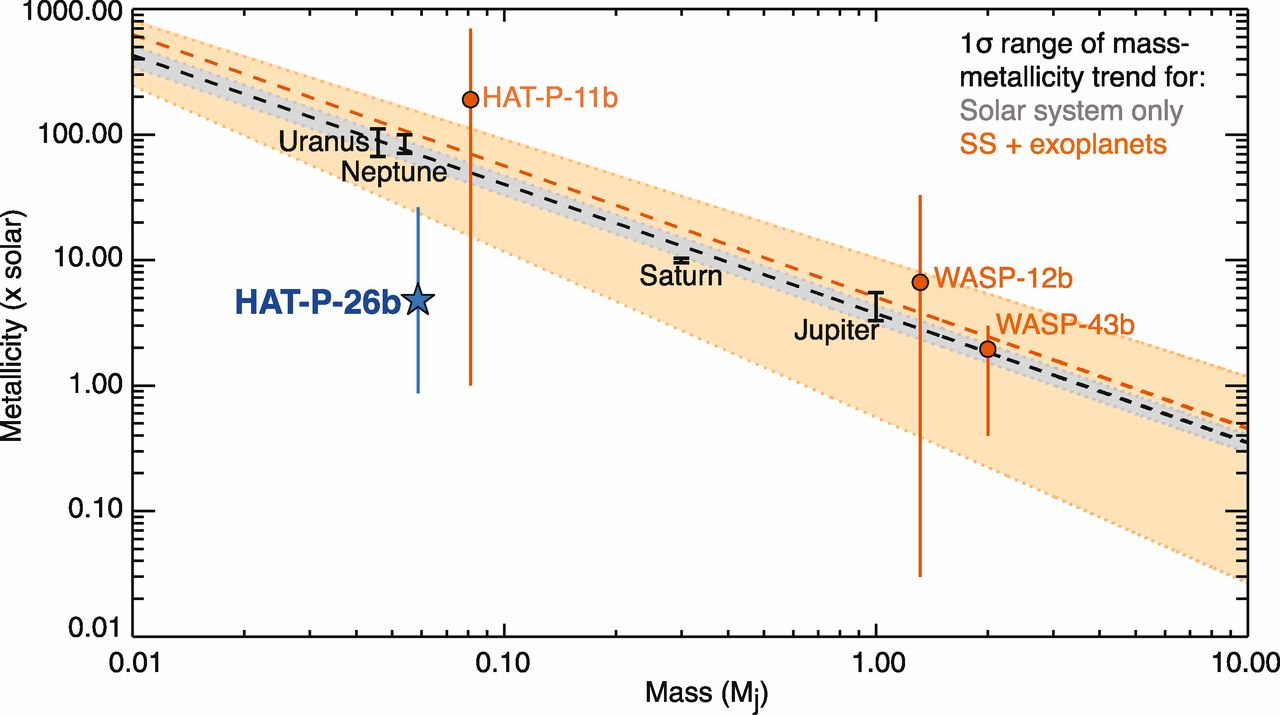
\includegraphics[scale=.8]{Figures/wakeford.jpg}
\caption{Mass metallicity.}
\label{fig:massZ}       
\end{centering}
\end{figure}

\runinhead{Abundance Ratios}
In addition to absolute abundances, abundance \emph{ratios} also constrain planet origins \citep{FIXME}. These ratios are sensitive to the planet's formation location: as the disk temperature drops with radial distance from the star, molecules reach their freezing points, beginning with H$_2$O and followed by CO$_2$ and CO \citep{oberg11}. These frost lines lead to variation in abundance ratios for gas versus solid material which can be imprinted on the composition of forming planets \citep{madhusudhan14, alidib16, mordasini16}.

The most common measure of a planet's abundance pattern is its carbon-to-oxygen ratio (C/O). enhanced \citep{madhusudhan12}.  Despite early evidence for a carbon-rich atmospheric composition for WASP-12b \citep{madhusudhan11}, further scrutiny of hot Jupiters has revealed $\mathrm{C/O} < 1$ in all cases \citep{line14, kreidberg15b, benneke15, barstow17}.  These measurements agree well with planet formation theory, which predicts C/O  \citep[e.g.][]{madhusudhan14, mordasini16}. Planet formation models More precise estimates of C/O and other ratios will be possible with future instruments that have spectroscopic coverage of additional molecules. 


\subsection{Climate}
With thermal emission measurements, it is possible to characterize a planet's climate in detail.  Nearly all of these observations have focused on hot Jupiters with large planet-to-star flux ratios. The most common measurement is of dayside brightness temperature, which has been inferred from secondary eclipse observations for over 50 planets \citep{schwartz15}. Measured dayside temperatures range from roughly 1000 to 3000 K \citep{stevenson14b, kammer15, morley17}.  Cooler planets will be more accessible with future instruments that are sensitive to longer wavelength photons.

\runinhead{Thermal Inversions}
One can also determine the atmosphere's \hbindex{temperature-pressure profile} using emission spectroscopy. At wavelengths where the atmosphere has higher opacity, the emitted light comes from higher altitudes. The spectrum is therefore sensitive to thermal structure.  Early \Spitzer\ observations of HD 209458b suggested the atmosphere had an inverted thermal profile, where temperature increased with height \citep{knutson08}. Such \hbindex{thermal inversions} can result from upper atmosphere heating by a strong optical or UV absorber (for example, Earth's stratosphere is due to ozone absorption).  Further observations of HD 209458b showed that it does not in fact have a thermal inversion \citep{diamond-lowe14, schwarz15}. However, there is new evidence for weak thermal inversions (isothermal profiles) in the atmospheres of other planets \citep{stevenson14, haynes15}.
 

\runinhead{Global Heat Circulation}
Thermal phase curves provide additional insight into global recirculation.
The first spectroscopic phase curve was obtained for the hot Jupiter WASP-43b.  
hot spot offset - winds


\subsection{Aerosols}
\hbindex{Aerosols} -- an umbrella term for clouds and hazes -- are ubiquitous in the Solar System and are proving to be common in exoplanets as well. Transmission spectra are particularly sensitive to the presence of aerosols, due to the slant viewing geometry observed during transit \citep{fortney05}.  Aerosols have three main effects on transmission spectra:  first, they truncate absorption features (as illustrated in Figure FIXME).  They can also introduce a slope in the spectrum over wavelength intervals of several microns \citep[e.g][]{sing16}.  The third effect is scattering off cloud and haze particles at optical wavelengths, which introduces a steep increase in transit depth towards the blue \citep[e.g.][]{pont08}.

The first hint of extrasolar aerosols came from HD 209458b, which had a smaller than expected sodium feature relative to a clear atmosphere \citep{charbonneau02}. This observation foreshadowed a slew of spectra with truncated features \citep[e.g.][]{deming13, crossfield13, kreidberg14a, knutson14a, kreidberg15b}. Many spectra have also shown the large optical slope indicative of scattering from small particles \citep[e.g][]{sing11, sing13, robinson14, dragomir15}. Transit depth offsets between 1 and 5 $\mu$m are also seen in many hot Jupiters \citep{sing16}.

Despite this body of evidence, the makeup of the aerosols has proven elusive. There are a number of theoretical possibilities, including equilibrium condensates such as water, salt, sulfide, or silicate clouds (depending on temperature) and photochemical hazes, e.g. hydrocarbon soots formed from photolyzed methane \citep{burrows99, kempton12, morley13, wakeford17}. Current transmission spectra lack the wavelength coverage and precision needed to distinguish between these species in exoplanets.  In brown dwarfs, a silicate feature at 9 $\mu$m has been tentatively detected using \Spitzer/IRS \citep{cushing06}. Future observations of exoplanets could also reveal features from specific grains, which would unambiguously determine their composition \citep{wakeford15}.

Meanwhile, there are several indirect constraints on aerosol properties.  For example, optical phase curves of hot Jupiters are best explained by reflective clouds on their western hemispheres, composed of silicate or manganese sulfide \citep{demory13, oreshenko16, parmentier16}. Further clues come from the amplitude of spectral features. For example, the spectrum of the super-Earth GJ 1214b is featureless at high precision \citep[30 ppm,][]{kreidberg14a}.  Truncating the features to this extent requires an optically thick aerosol layer at a pressure level of 0.1 millibar, which can be achieved either by thick, lofted clouds or very efficient haze formation \citep{morley15}. 

Demographics:
There is some evidence that aerosols are more prevalent at lower temperatures \citep{stevenson16, heng16}. surface grav? FIXME

\section{Future Prospects}
We are on the threshold of a revolution in exoplanet atmosphere characterization thanks to several upcoming observing facilities.  The first of these is the Transiting Exoplanet Survey Satellite (\TESS), a planet finding mission scheduled to launch in 2018 \citep{ricker14}.  The goal of \TESS\ is to search 200,000 of the brightest stars in the sky for transiting planets, with an expected yield of nearly 2000 discoveries \citep{sullivan15}. In contrast to the majority of transiting planets discovered to date by \Kepler, the \TESS\ planets will have bright enough host stars for precise atmosphere characterization. The sample will also include smaller and cooler planets than are typically discovered by ground-based surveys of bright stars. 

The second game-changer is \JWST. The primary technical limitations in atmosphere characterization thus far have been aperture size and wavelength coverage, and \JWST\ offers major improvements on both fronts. It has roughly ten times the collecting area of \HST\, and provides spectroscopy from the optical to the infrared ($0.6 - 28\,\mu$m). The improvement in precision will make it possible to push down to sub-Neptune and smaller planets, and to study giant planets with unprecedented S/N. The expanded wavelength coverage will also enable the first spectroscopic detections of many molecules which have been elusive so far (including methane, carbon dioxide, and ammonia). Finally, \JWST's infrared detector MIRI will be sensitive to thermal emission from cooler objects, including potentially habitable worlds.

\runinhead{Pushing to Earth-Like Planets}
Atmosphere characterization for terrestrial planets is a challenge, but it is easiest for planets transiting nearby small stars.  Fortunately, such planets are common: roughly a quarter of M-dwarfs host a terrestrial planet in the habitable zone \citep{dressing15}. A number of these have been detected already, included three of the seven planets around the ultra-cool dwarf star TRAPPIST-1 and LHS 1140b \citep{gillon17, dittmann17}. Assuming these planets have Earth-like compositions, the expected amplitude of spectral features in their atmospheres is FIXME -- a goal within reach of an intensive JWST observing campaign with repeated transit and eclipse observations of each planet.  JWST is scheduled to launch in early 2019, and may provide us with the first ever constraints on terrestrial planet atmospheres beyond the Solar System. 

\section{Bibliography}

\begin{acknowledgement}
The author acknowledges support from the Harvard Society of Fellows and the Harvard Astronomy Department Institute for Theory and Computation. She is grateful for helpful comments from Caroline Morley, Hannah Diamond-Lowe, and Tyler Robinson.
\end{acknowledgement}

\bibliographystyle{spbasicHBexo}  %for bibtex
\bibliography{chapter} %for bibtex-example

\end{document}

